\documentclass[11pt]{beamer}
\usetheme[progressbar=frametitle]{metropolis}
\usepackage{xcolor} %Farbe überschriften
\definecolor{blue}{RGB}{24,116,190}
\setbeamercolor{progress bar}{fg=blue}

%\usecolortheme{owl}

\usepackage{appendixnumberbeamer}
\usepackage[utf8]{inputenc}
\usepackage[T1]{fontenc}
\usepackage{graphicx}
\usepackage{lmodern}
%\usepackage{beamercolorthemeowl}
\usepackage{pgfpages}
%\setbeameroption{show notes} %Notizen anzeigen
%\setbeameroption{show notes on second screen}
\makeatletter
\setlength{\metropolis@progressinheadfoot@linewidth}{3pt}
\setlength{\metropolis@titleseparator@linewidth}{1pt}
\setlength{\metropolis@progressonsectionpage@linewidth}{3pt}

\author{Laura Hartzheim}

\title{Arten des Machine Learnings - Supervised, Unsupervised und Reinforcement Learning}

\subtitle{}

\logo{}

\institute{}

\date{}

\subject{}

\setbeamercovered{transparent}

\setbeamertemplate{navigation symbols}{}

\begin{document}
	
	
	\begin{frame}
		\titlepage
	\end{frame} 
	
	\begin{frame}
		\frametitle{Inhalt}
		\tableofcontents
	\end{frame} 
	
	\section{Machine Learning}
	\begin{frame}
		\frametitle{Was ist Machine Learning?}
		\begin{itemize}
			\item Schnittmenge aus Statistik, Künstlicher Intelligenz und Informatik
			\item Maschine soll aus Daten lernen können, durch Erfahrung und Leistungsmessung
			%Bsp spam filter
		\end{itemize} 
	\end{frame}
	
	\begin{frame}
		\frametitle{Warum nutzt man Machine Learning?}
		\begin{itemize}
			\item vereinfachter Code und bessere Performanz bei Problemen mit vielen Regeln, da Regeln von Machine gelernt werden 
			\item Programme leichter zu warten und weniger fehleranfällig
			\item bietet Lösungen für komplexe Probleme die durch normale Programme nicht lösbar sind
			\item und vieles mehr
			%Email bsp
			
		\end{itemize} 
	\end{frame}
	
	\section{Supervised Learning}
	
	\begin{frame}
		\frametitle{Supervised Learning}
		\begin{itemize}
			\item Nutzen von bekannten Daten und Ausgaben(Label) während des Trainings 
			\item Ziel: eingehende Daten den entsprechenden ausgehenden Daten zuzuordnen
			% Over und Underfitting ?
		\end{itemize}
	\end{frame}
	
	\begin{frame}
		\frametitle{Klassifikation}
		\begin{itemize}
			\item Ziel: Klassenlabel für die eingehenden Daten voraussagen
			\item binäre Klassifikation: nur zwei mögliche Label $\rightarrow$ Ja/Nein-Frage
			\item multiklassen Klassifikation: mehrere Klassen möglich
			\item Erstellen von Regeln während der Trainings-Phase 
		\end{itemize}
		
	\end{frame}
	
	\begin{frame}
		\frametitle{Klassifikation}
		\centering
		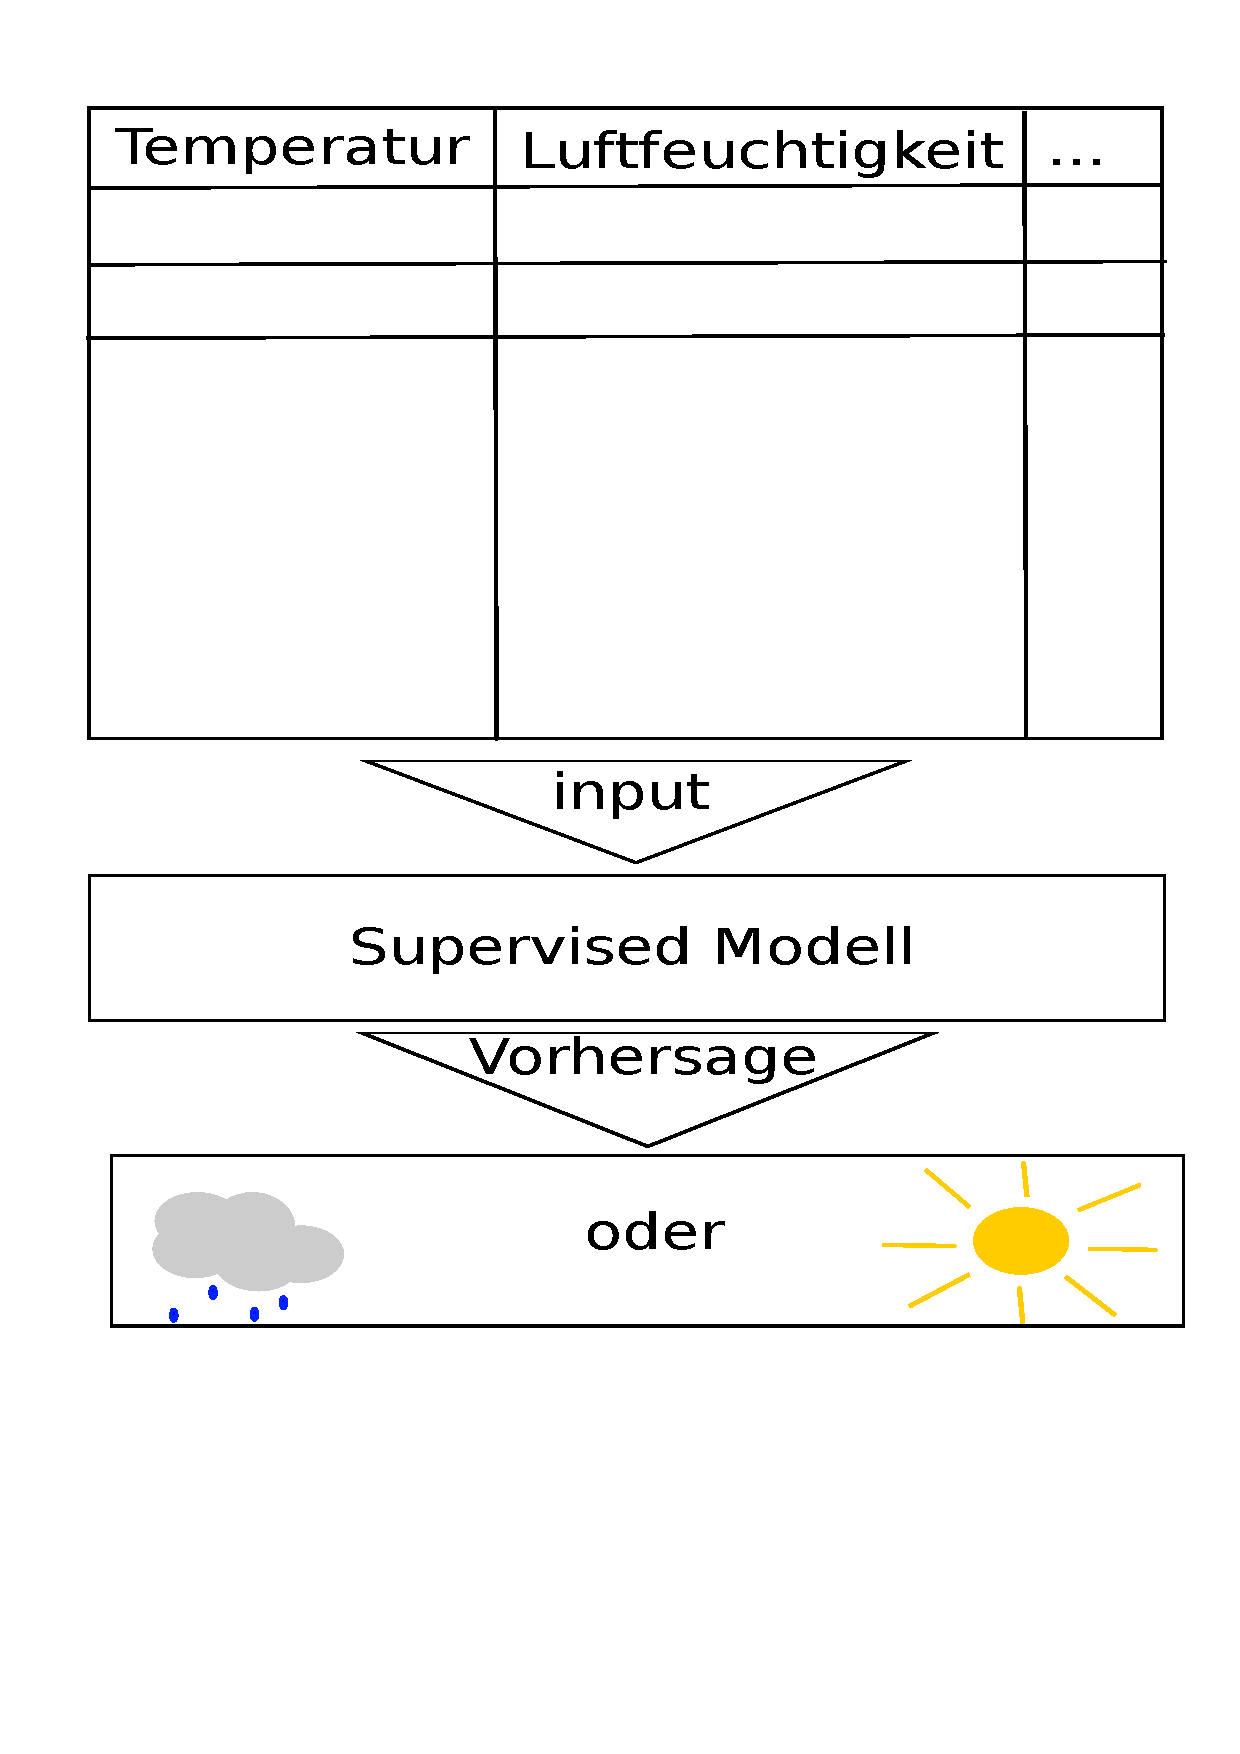
\includegraphics[width=200pt]{C:/Users/Laura/Documents/GitHub/LaTexSeminar/bilder/Label.pdf}
	\end{frame}
	
	\begin{frame}
		\frametitle{Regression}
		\begin{itemize}
			\item Ziel: Ermitteln von Werten
			\item keine Klassen
			\item lernen der Zusammenhangs der In- und Output Daten
			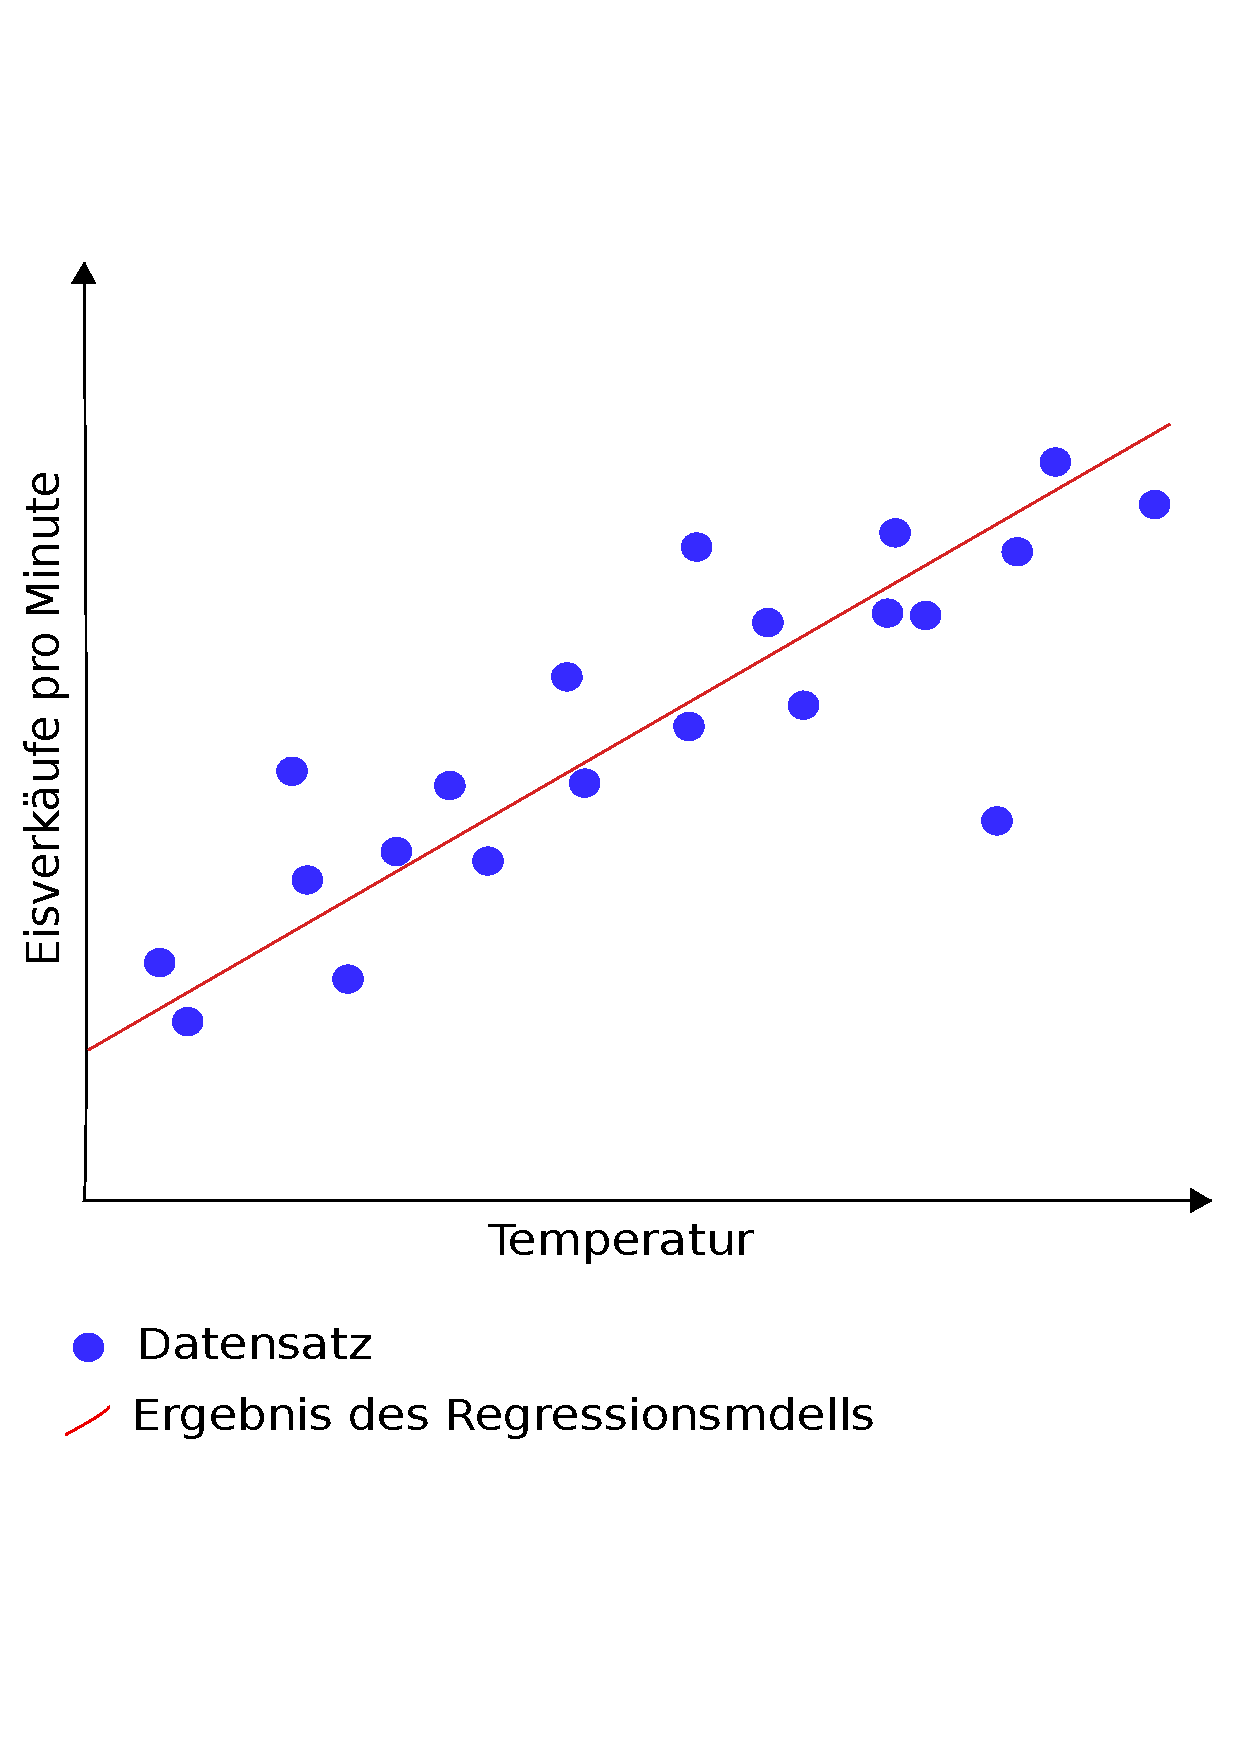
\includegraphics[width=200pt]{C:/Users/Laura/Documents/GitHub/LaTexSeminar/bilder/Regression.pdf}
		\end{itemize}
		
	\end{frame}
	
	\section{Unsupervised Learning}
	
	\begin{frame}
		\frametitle{Unsupervised Learning}
		\begin{itemize}
			\item keine bekannten Output-Daten/Label beim Training
			\item schwer feststellbar ob Modell korrekte Ergebnisse erzielt
			\item Maschine bekommt Input-Daten und muss anhand dieser Entscheidungen treffen und kategorisieren
			\item Modell lernt Muster, Strukturen und Beziehungen in Datensätzen
		\end{itemize}
	\end{frame}
	
	\begin{frame}
		\frametitle{Clusterbildung}
		\begin{itemize}
			\item Ziel: in jedem Cluster möglichst ähnliche Daten, die sich zu Daten aus anderen Clustern unterscheiden
			\item Clusterbildung durch Muster, Ähnlichkeiten und Verbindungen zwischen Datensätzen
		\end{itemize}
		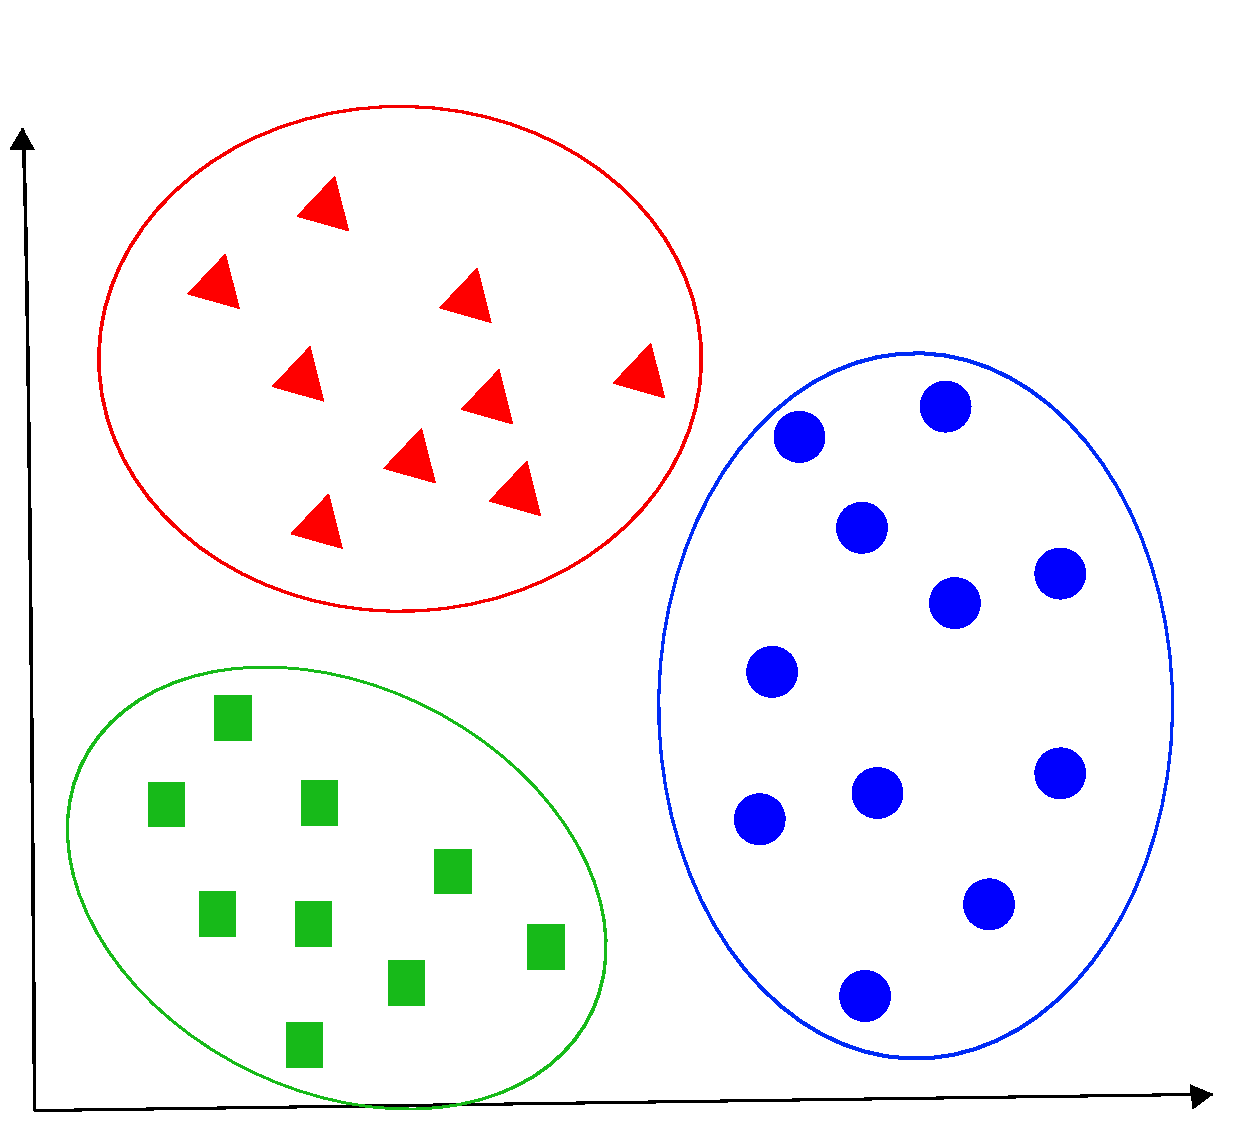
\includegraphics[width=130pt]{C:/Users/Laura/Documents/GitHub/LaTexSeminar/bilder/Cluster.pdf}
	\end{frame}
	
	\begin{frame}
		\frametitle{Dimensionsreduktion}
		\begin{itemize}
			\item Komplexität des Modells ist abhängig von der Anzahl der Inputs
			\item Ziel: Input Space(= Anzahl der Features/Attribute) verkleinern
			\item Feature Extraction: neue Features, die Kombinationen aus alten sind finden 
			\item Feature Selection: 
				\begin{itemize}
					\item k Dimensionen aus d auswählen durch Subset Selection
					\item Features die die meisten Informationen liefern werden ausgewählt, der Rest verworfen
					\item keine neuen Features
					\item Ziel Subset Selection: bestes Subset aus Features mit möglichst geringer Anzahl an Dimensionen und bester Genauigkeit
				\end{itemize}
		\end{itemize}  
	\end{frame}
	
%	\begin{frame}
%		\frametitle{Anomalie Erkennung}
%		\begin{itemize}
%			\item Ziel: seltene oder laut vorherigen Datensätzen untypische Ereignisse erkennen
%			\item Anomalien können nach bestimmten Mustern auftreten
%			\item in der Trainings-Phase haben alle Input-Daten keinen Anomalien
%		\end{itemize}
%		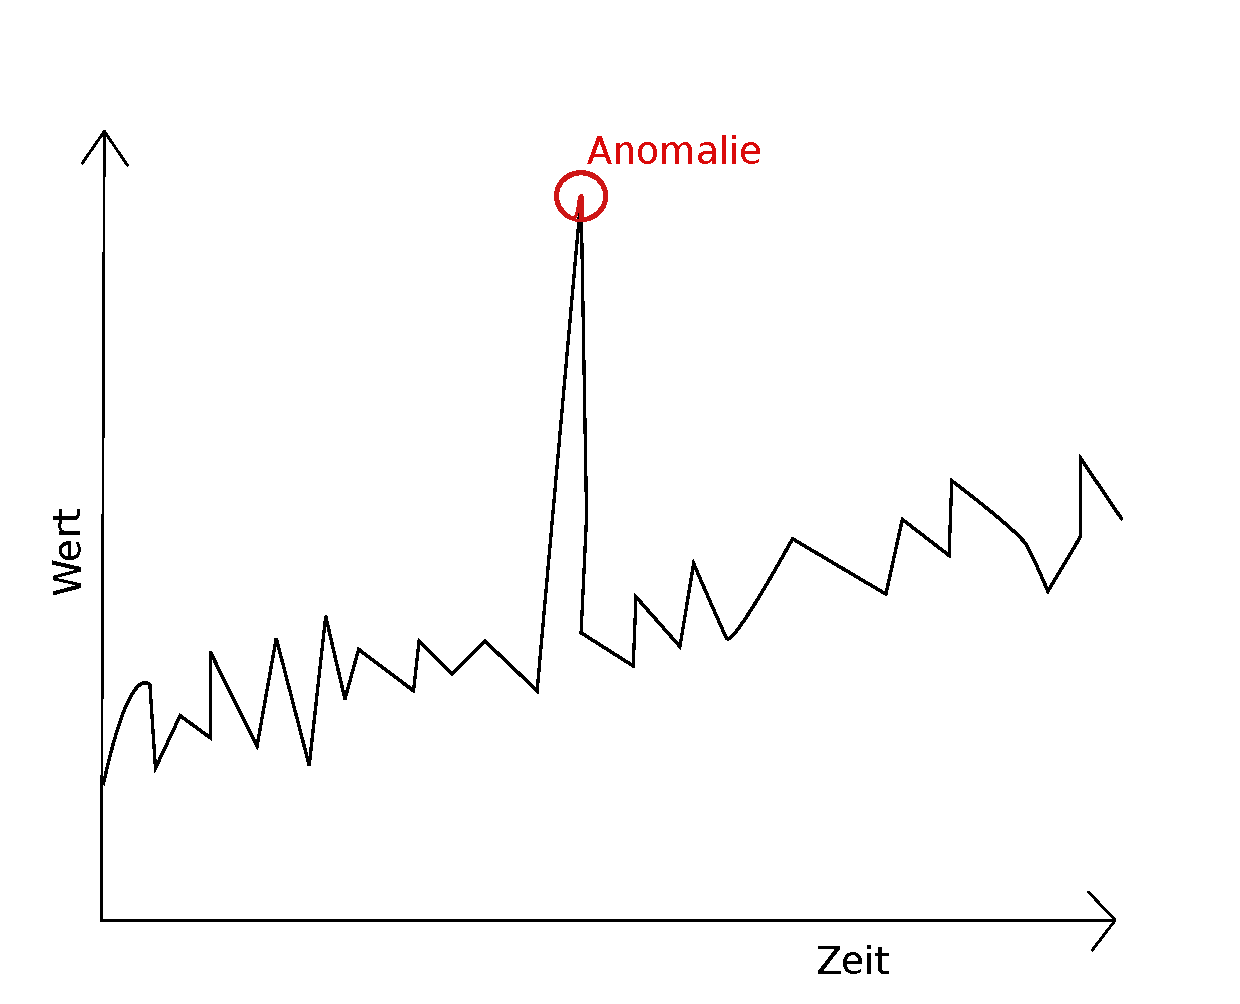
\includegraphics[width=170pt]{C:/Users/Laura/Documents/GitHub/LaTexSeminar/bilder/Anomalie.pdf}
%	\end{frame}
%	
%	\begin{frame}
%		\frametitle{ Association rule-mining}
%		\begin{itemize}
%			\item Untersuchen und Analysieren von Transaktionen um Muster oder Regeln zu bestimmen
%			\item wird auch "market basket analysis" genannt
%			\item Ergebnisse z.B. für Produktvorschläge basierend auf dem eigenen Warenkorb und Käufen anderer Nutzer 
%		\end{itemize} 
%		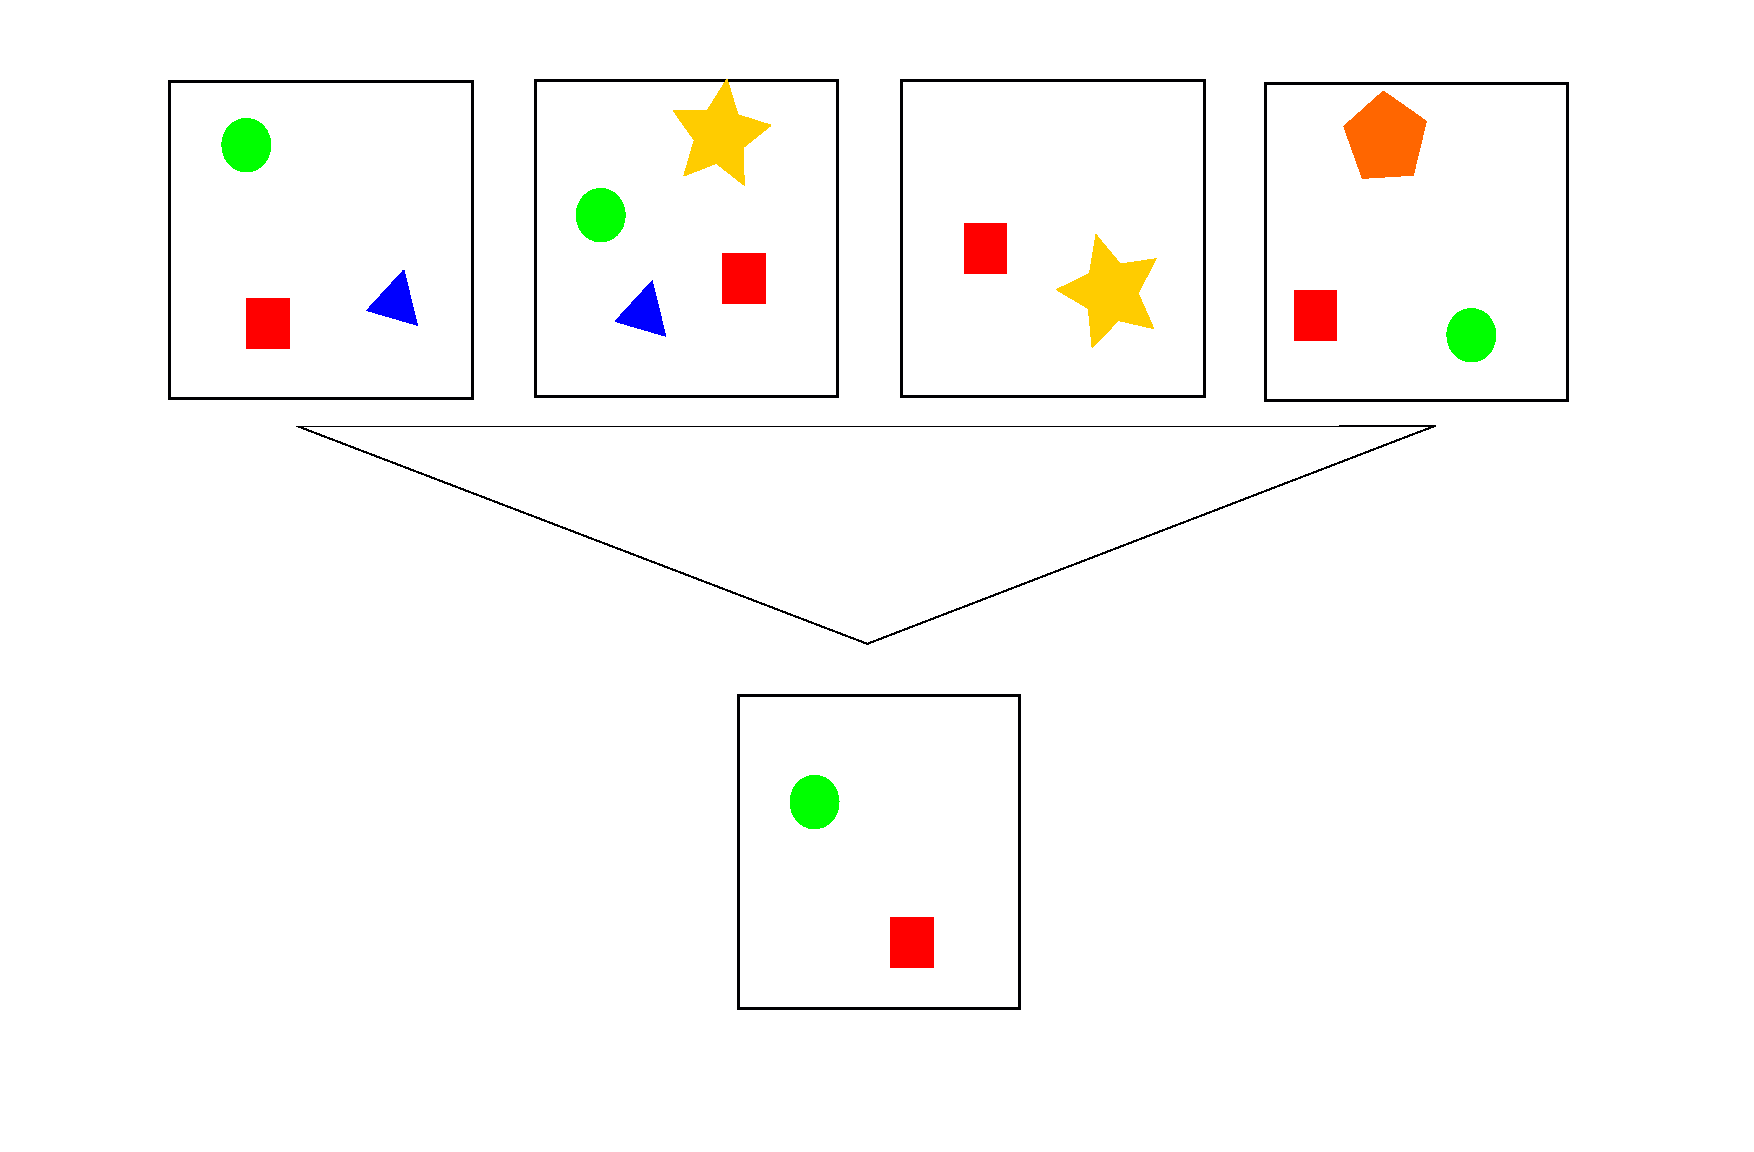
\includegraphics[width=170pt]{C:/Users/Laura/Documents/GitHub/LaTexSeminar/bilder/rule-mining.pdf}
%	\end{frame}
	
	\section{Reinforcement Learning}
	
	\begin{frame}
		\frametitle{Reinforcement Learning}
		\begin{itemize}
			\item Einsatz von Agenten $\widehat{=}$ intelligente Programme
			\item Agent trainiert um sich Umgebung anzupassen und seine Leistung zu verbessern
			\item Agent kennt Zustand der Umgebung und führt Aktionen aus um diesen zu verändern
			\item Agent hat Strategien und Richtlinien, die verbessert und angepasst werden
			\item Abhängig von der Aktion erhält der Agent positive und negative Belohnungen
		\end{itemize}
		\centering
		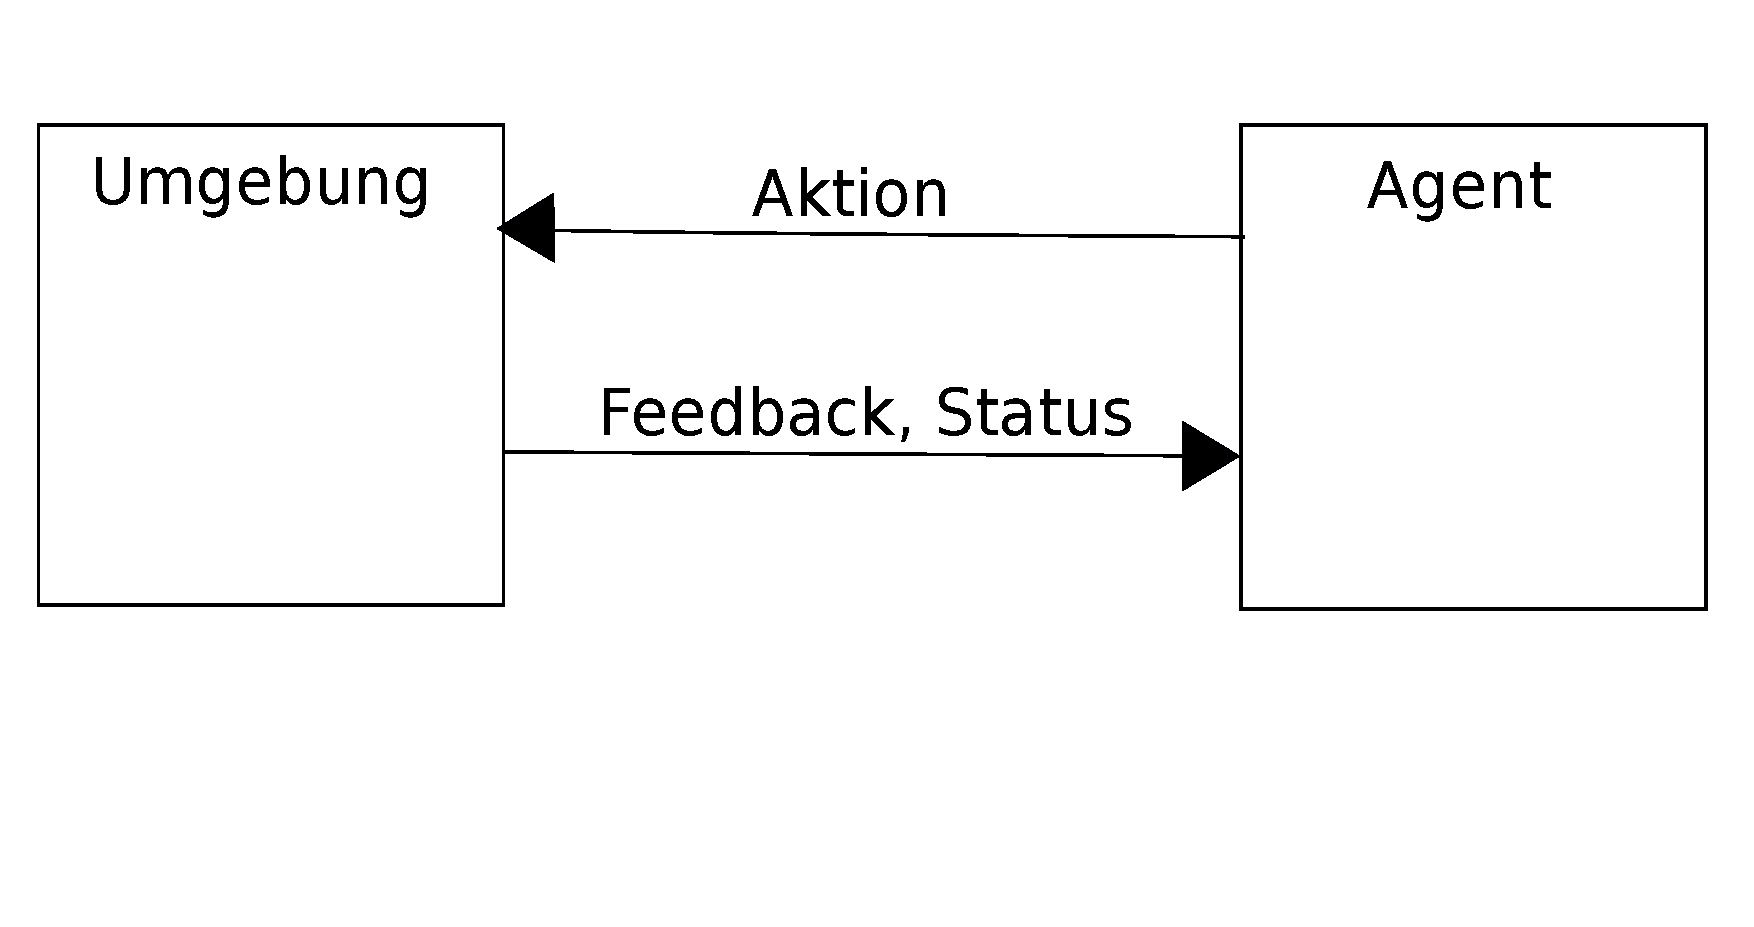
\includegraphics[width=180pt]{C:/Users/Laura/Documents/GitHub/LaTexSeminar/bilder/Reinforcement.pdf}
	\end{frame}
	
%	\begin{frame}
%		\frametitle{Umgebung}
%		\begin{itemize}
%			\item kann eine 2D oder 3D Simulation eines Szenarios aus der echten Welt oder aus einem Spiel sein
%			\item Eigenschaften:
%			\begin{itemize}
%				\item deterministisch: für jede Aktion nur ein Übergang anderem Zusatand möglich $\leftrightarrow$ nicht-deterministisch
%				\item beobachtbar: alle Informationen über die Umgebung sind bekannt/ können wahr genommen werden $\leftrightarrow$ teilweise beobachtbar %Poker und Schach bsp
%				\item fortlaufend: mehr als eine Aktion führt zum nächsten Zustand $\leftrightarrow$ beschränkt
%			\end{itemize}
%		\end{itemize}
%	\end{frame}
	
	\section{Fazit}
	
	\begin{frame}
		\frametitle{Fazit}
		\begin{itemize}
			\item Machine Learning Arten haben sehr unterschiedliche Nutzen
			\item Supervised Learning: Zuordnung in Kategorien und Abschätzung von Funktionen 
			\item Unsupervised Learning: Ergebnisse sind nicht immer die Lösung des Problems, oft unterstützend für Supervised Algorithmen
			\item Reinforcement Learning: großer Unterschied zu den anderen, Verhaltensmuster werden optimiert
		\end{itemize}
		$\Rightarrow$ Alle sind bedeutend, da sie sich für sehr verschiedene Problemstellungen eignen
		
	\end{frame}
	
	\section{Code}
	
	\begin{frame}
		\frametitle{Titelseite}
		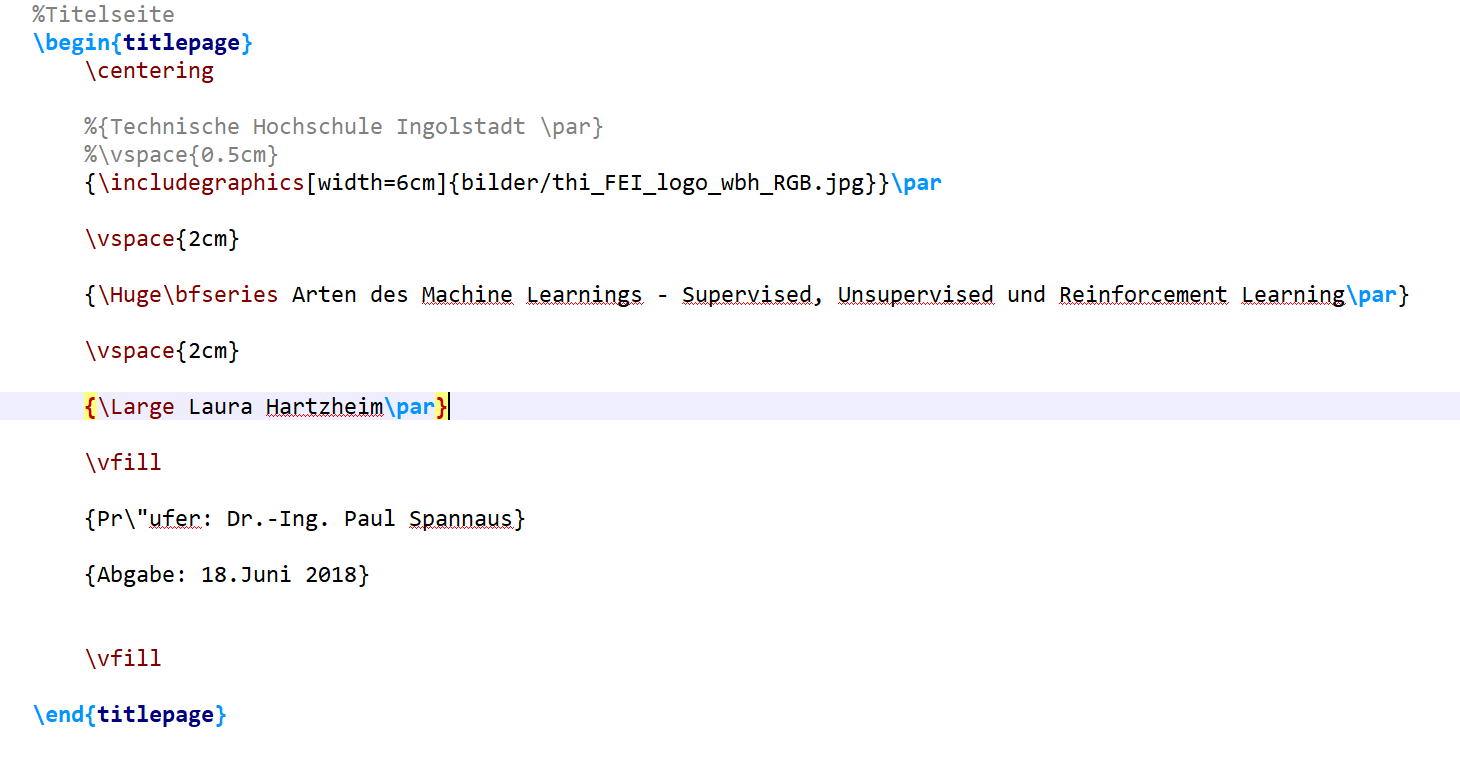
\includegraphics[width=350pt]{Titelseite.png}
	\end{frame}
	
	\begin{frame}
		\frametitle{Bildplatzierung}
		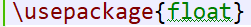
\includegraphics[width=90pt]{PackageH.png}
		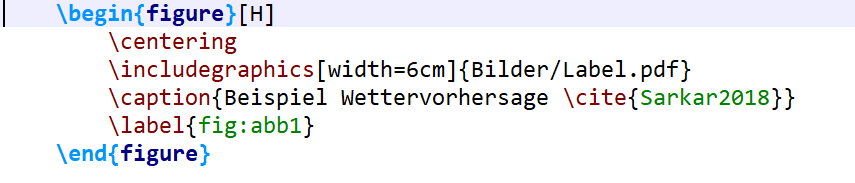
\includegraphics[width=300pt]{BildH.png}
	\end{frame}
	

\end{document}